\documentclass[tikz]{standalone}
\usepackage{amsmath}
\usepackage{times}
\usepackage{txfonts}

\usetikzlibrary{arrows}
\usetikzlibrary{intersections}
\usetikzlibrary{math}
\usetikzlibrary{positioning}
\usetikzlibrary{arrows.meta}
\usetikzlibrary{shapes.misc}
\usetikzlibrary{calc}

\begin{document}
  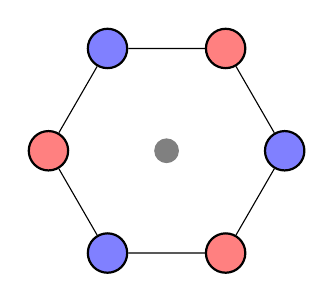
\begin{tikzpicture}[
      >=latex, 
      node distance = 2mm,
      charge/.style = {
        circle, draw = black, thick,
        minimum size = 5mm
      },
      positive/.style = { fill = red!50 },
      negative/.style = { fill = blue!50 },
    ]

    \foreach \x/\t [count=\i] in {60/positive, 120/negative, 180/positive, 240/negative, 300/positive, 360/negative} {
      \node[charge, \t] (C\i) at (\x:1.5cm) {};
    }

    \draw[black] (C1) to (C2) to (C3) to (C4) to (C5) to (C6) to (C1);
    \node[circle, draw=gray, fill=gray, outer sep = 0, inner sep = 0, minimum size = 3mm] {};
    % \draw[gray, dashed] (C2) to (C4) to (C6) to (C2);
  \end{tikzpicture}
\end{document}
